
\documentclass{article}
\usepackage[ascii]{inputenc}
\usepackage[T1]{fontenc}
\usepackage[english]{babel}
\usepackage{amsmath}
\usepackage{amssymb,amsfonts,textcomp}
\usepackage{color}
\usepackage{array}
\usepackage{supertabular}
\usepackage{hhline}
\usepackage[normalem]{ulem}
\usepackage{hyperref}
\usepackage{textcomp}
\usepackage{layout}
\usepackage[numbers]{natbib}
\usepackage{caption}

\hypersetup{colorlinks=true, linkcolor=black, citecolor=black, filecolor=blue, urlcolor=blue, pdftitle=CAD17abstract, pdfauthor=Orest Mykhaskiv, pdfsubject=, pdfkeywords=}
\usepackage[pdftex]{graphicx}

\newcommand\textstyleInternetlink[1]{\textcolor{blue}{#1}}

\setcounter{secnumdepth}{2}
\renewcommand\thesection{\arabic{section}}
\renewcommand\thesubsection{\arabic{section}.\arabic{subsection}}
\makeatletter
\newcommand\arraybslash{\let\\\@arraycr}
\makeatother

\newcommand\liststyleWWviiiNumxxxiii{%
\renewcommand\labelitemi{{\textbullet}}
\renewcommand\labelitemii{{}-}
\renewcommand\labelitemiii{${\blacksquare}$}
\renewcommand\labelitemiv{{\textbullet}}
}
\newcommand\liststyleWWviiiNumxxix{%
\renewcommand\labelitemi{{\textbullet}}
\renewcommand\labelitemii{o}
\renewcommand\labelitemiii{${\blacksquare}$}
\renewcommand\labelitemiv{{\textbullet}}
}
\newcommand\liststyleWWviiiNumxxiv{%
\renewcommand\labelitemi{{\textbullet}}
\renewcommand\labelitemii{o}
\renewcommand\labelitemiii{${\blacksquare}$}
\renewcommand\labelitemiv{{\textbullet}}
}
\newcommand\liststyleWWviiiNumxxi{%
\renewcommand\labelitemi{{\textbullet}}
\renewcommand\labelitemii{o}
\renewcommand\labelitemiii{${\blacksquare}$}
\renewcommand\labelitemiv{{\textbullet}}
}
\newcommand\liststyleWWviiiNumxxiii{%
\renewcommand\labelitemi{{\textbullet}}
\renewcommand\labelitemii{o}
\renewcommand\labelitemiii{${\blacksquare}$}
\renewcommand\labelitemiv{{\textbullet}}
}
\newcommand\liststyleWWviiiNumxv{%
\renewcommand\labelitemi{{\textbullet}}
\renewcommand\labelitemii{o}
\renewcommand\labelitemiii{${\blacksquare}$}
\renewcommand\labelitemiv{{\textbullet}}
}
\newcommand\liststyleWWviiiNumxxx{%
\renewcommand\theenumi{\arabic{enumi}}
\renewcommand\theenumii{\alph{enumii}}
\renewcommand\theenumiii{\roman{enumiii}}
\renewcommand\theenumiv{\arabic{enumiv}}
\renewcommand\labelenumi{[\theenumi]}
\renewcommand\labelenumii{\theenumii.}
\renewcommand\labelenumiii{\theenumiii.}
\renewcommand\labelenumiv{\theenumiv.}
}
\newcommand\liststyleWWviiiNumxxxii{%
\renewcommand\labelitemi{{\textbullet}}
\renewcommand\labelitemii{o}
\renewcommand\labelitemiii{${\blacksquare}$}
\renewcommand\labelitemiv{{\textbullet}}
}

\renewcommand\refname{}
\renewcommand{\bibsection}{}
\renewcommand{\theequation}{2.\arabic{equation}}


\setlength\paperwidth{19.05cm}
\setlength\paperheight{26.162cm}
\setlength\voffset{-1in}
\setlength\hoffset{-1in}
\setlength\topmargin{30pt}
\setlength\oddsidemargin{1.524cm}
\setlength\textheight{576pt}
\setlength\textwidth{16.001999cm}
\setlength\footskip{0.841cm}
\setlength\headheight{16pt}
\setlength\headsep{28pt}


\usepackage{fancyhdr}
\pagestyle{fancy}
\fancyhf{}
\renewcommand{\headrulewidth}{0pt}
\renewcommand{\footrulewidth}{0.4pt}
\fancyhead[R]{\thepage}
\fancyfoot[R]{Proceedings of CAD'21, Barcelona, Spain, July 5-7, 2021, aaa-bbb\\ {\footnotesize{\textcopyright}} 2021 CAD Solutions, LLC, \ULurl{http://www.cad-conference.net}}

\usepackage{etoolbox}
\patchcmd{\thebibliography}{\section*{\refname}}{}{}{}
\captionsetup[figure]{labelformat={default},name={Fig.}}

\setlength{\bibsep}{2pt plus 0.3ex}
\setcounter{page}{1}

\makeatletter
\DeclareUrlCommand\ULurl@@{%
  \def\UrlFont{\ttfamily\color{blue}}%
  \def\UrlLeft{\uline\bgroup}%
  \def\UrlRight{\egroup}}
\def\ULurl@#1{\hyper@linkurl{\ULurl@@{#1}}{#1}}
\DeclareRobustCommand*\ULurl{\hyper@normalise\ULurl@}
\makeatother

\begin{document}

{\centering  
\includegraphics[width=5.173cm,height=2.193cm]{images/CADconverted-img001.jpg} \par}

\vspace{5pt}
\noindent
\underline{Title:}

\noindent{\bfseries
Word Template for CADxx Extended Abstracts }

\vspace{1em}
\noindent \underline{Authors:}
\newline
John C. Gotti, gotti@cityuny.edu, City University of New York \newline
Jessie A. James, Jessie@tsu.edu, Texas State University \newline
Donald L. Corleone, don@dlc.com, 3DLC and Associates

\vspace{1em}
\noindent \underline{Keywords:}\newline
Rapid Prototyping, FDM, Z-Printer, Surface Finish, Dimensional Accuracy, Process Optimization


\bigskip


\noindent \underline{DOI:} 10.14733/cadconfP.2021.xxx-yyy

\vspace{10pt}
\noindent\underline{Introduction:}\vspace{0.2em}\newline
In engineering workflows it is common practice to maintain master CAD geometries, which then serve as a foundation for further design and development. Preserving CAD parametrisations during aerodynamic shape optimisation becomes challenging since existing CAD tools do not provide derivatives necessary for gradient-based design methods. Hence, gradients are obtained by approximations or with simplifications, precluding full CAD integration into the design optimisation loop.

 
In the present work, we obtain exact CAD sensitivities (derivatives) with respect to CAD design parametrisation using our algorithmically differentiated Open Cascade Technology (OCCT) CAD-kernel software.  The extension of this software for optimisation of parametric models and BRep (NURBS) compose the tool for explorations of the optimal shape in different by size and nature design spaces. In addition, we demonstrate the imposition of geometric constraints for both approaches, a salient part of industrial design, and an intuitive method of storing them in standard CAD format.\newline


\textbf{This template file is courtesy of Orest Mykhaskiv, Jens-Dominik M\"uller, Pavanakumar Mohanamuraly, Mladen Banovic, Andrea Walther, Salvatore Auriemma and Herve Legrand.}


\vspace{10pt}
\noindent\underline{CAD-based Shape Optimisation:}\vspace{0.2em}\newline
To assess the aerodynamic performance of a given CAD geometry with design parameters $\alpha$, one usually computes a scalar cost function $J$ (drag, lift, total pressure loss, etc.) on the corresponding computational mesh.  In order to obtain a shape with improved characteristics we consider an optimisation problem \cite{jameson88aerodynamic}:       
\begin{equation}
\label{eq:cost-func}
\underset{\alpha}{min} \hspace{0.5em} J(U(X(\alpha)), X(\alpha), \alpha)
\end{equation}
\begin{equation}
\label{eq:NS}
R(U(X(\alpha)), X(\alpha)) = 0\:. 
\end{equation}
Equation \eqref{eq:NS} describes the flow field within the domain of interest by system of Reynolds-Averaged Navier-Stokes equations, with the state variable $U$ and computational mesh coordinates $X$, which depend on design parameters $\alpha$. In case of large amount of design parameters (usually the case in industrial applications) the adjoint method proves to be computationally efficient and could be derived by application of a chain rule to the system \eqref{eq:cost-func}-\eqref{eq:NS} yielding:
\begin{equation}
\label{eq:sens}
\dfrac{dJ}{d\alpha}=\Big[ \frac{dJ}{dX} +\nu^Tf \Big]\frac{\partial X}{\partial \alpha}\:,
\end{equation}
where 
\begin{equation}
f = -\frac{\partial R}{\partial X}\:.
\end{equation}
Here $\nu$ represents the solution of adjoint equations:
\begin{equation}
\label{eq:adjoint}
\Big ( \frac{\partial R}{\partial U}\Big)^T\nu=\frac{\partial J}{\partial U}\:.
\end{equation}
After computing the solution of primal and adjoint equations \eqref{eq:NS},\eqref{eq:adjoint}, one can rewrite cost function gradient in terms of surface grid points derivatives:
\begin{equation}
\label{eq:surfSens}
\frac{dJ}{d\alpha}=\frac{dJ}{dX_S}\frac{dX_S}{d\alpha}\:.
\end{equation}
Here, the relation (spring analogy, inverse distance weighting) between volume and surface grid points displacement is used $X = X(X_S)$. 
The first term in \eqref{eq:surfSens}, usually called \textit{CFD sensitivity}, corresponds to the flow sensitivity in the surface grid points $X_S$. These derivatives could be calculated by several available CFD solvers that have implemented the adjoint method. In this work we use our in-house discrete adjoint solver STAMPS (previously \textit{mgopt}) \cite{xu2015thesis}. 

The second term (\textit{CAD sensitivity}) represents the derivative of the surface grid points $X_S$ with respect to the CAD model design parameters. This part is calculated in the automatically differentiated version of OCCT \cite{auriemma2016optimisation}. Although the process of differentiation of the complete CAD system was time-consuming and involved comprehensive code modifications (due to the size and complexity of the software), the final result is extremely beneficial for the CAD-based optimisation. The differentiated OCCT provides the derivatives for almost every possible CAD parametrisation and geometrical manipulation. 

Equipped with these derivatives, we compose them in the total gradient, which is then used in iterative gradient-based optimisation loop:
\begin{equation}
\alpha^{(n+1)} =  A\big(\alpha^{(n)}, \frac{dJ}{d\alpha}(\alpha^{(n)})\big) \:,\end{equation}
with $A$ as an optimisation algorithm. 
Next sections describe two cases of the above mentioned method, depending on the nature of CAD design parameter $\alpha$: as design variable in parametric CAD model or BRep/NURBS parametrisation.



\vspace{10pt}
\noindent\underline{Parametric CAD-model Optimisation:}\vspace{0.2em}\newline
Parametric models are extremely popular in industry since they allow designers and engineers to map their intuition and experience on a set of familiar and conventional variables: e.g. blade thickness, fillet radius, wing span, etc. The OCCT kernel proposes large amount of methods for typical parametric model construction: starting from sketches with pre-defined sizes, construction of 2D curves to further 3D shapes manipulations, boolean operations, etc. The software architecture of the differentiated OCCT allows to build parametric models with no difference to the original version, but additionally is capable of providing the derivatives with respect to the used design parameters. 

Existence of a parametric CAD model creates a natural way to incorporate various geometrical constraints, since most of design variables are explicitly controlled by user-defined parametrisation. In the final paper, an example of parametric CAD model in differentiated OCCT will be presented (TU Berlin Stator testcase, see description below), as well as the results of aerodynamic shape optimisation subject to several geometrical constraints. 


\vspace{10pt}
\noindent\underline{BRep (NURBS-based) Optimisation and Constraints:}\vspace{0.2em}\newline
Alternatively to the previous section, instead of changing the parameters of the model's construction algorithm, one can directly modify the geometry of the resulting shape, so-called BRep (Boundary Representation). Changes to this BRep data (control points positions and weights of corresponding NURBS) eliminate the initial parametrisation, but propose richer design spaces compared to sometimes limited parametric models. Hence, this method serves better the ultimate goal of optimisation, potentially exploring non-conventional designs. The method is CAD-vendor independent, and requires only a generic CAD-file (STEP, IGES, etc.), eluding problems with parametrisation tree and making the optimisation more automatic. With method implementation in OCCT, one can easily and intuitively refine design space by adding extra control points. 
\begin{figure}[t!]
\label{fig:constraint}
\begin{center}
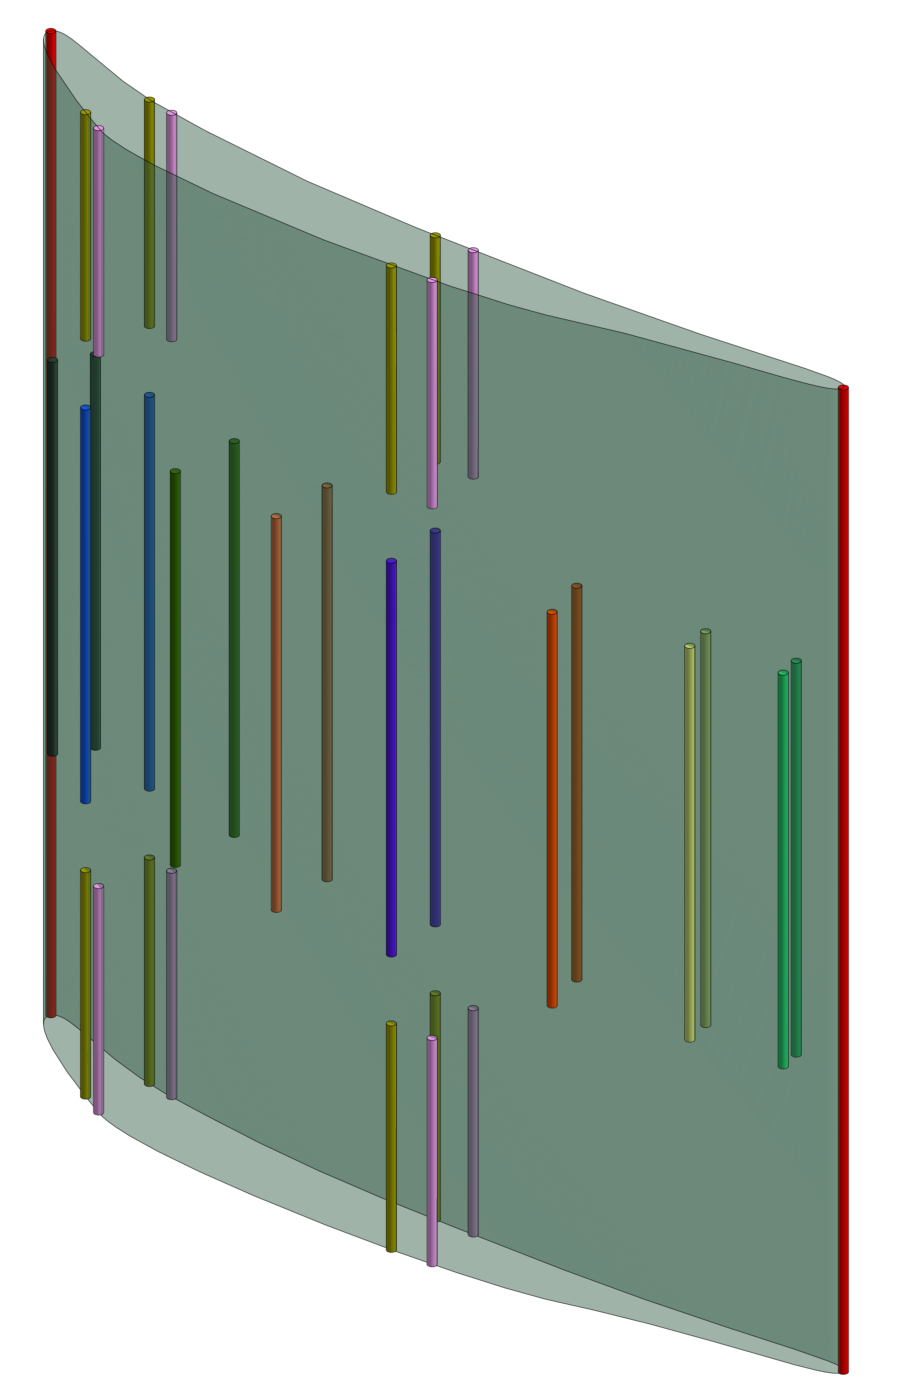
\includegraphics[width = 0.3\textwidth]{images/NewCylindersC1.pdf}
~~

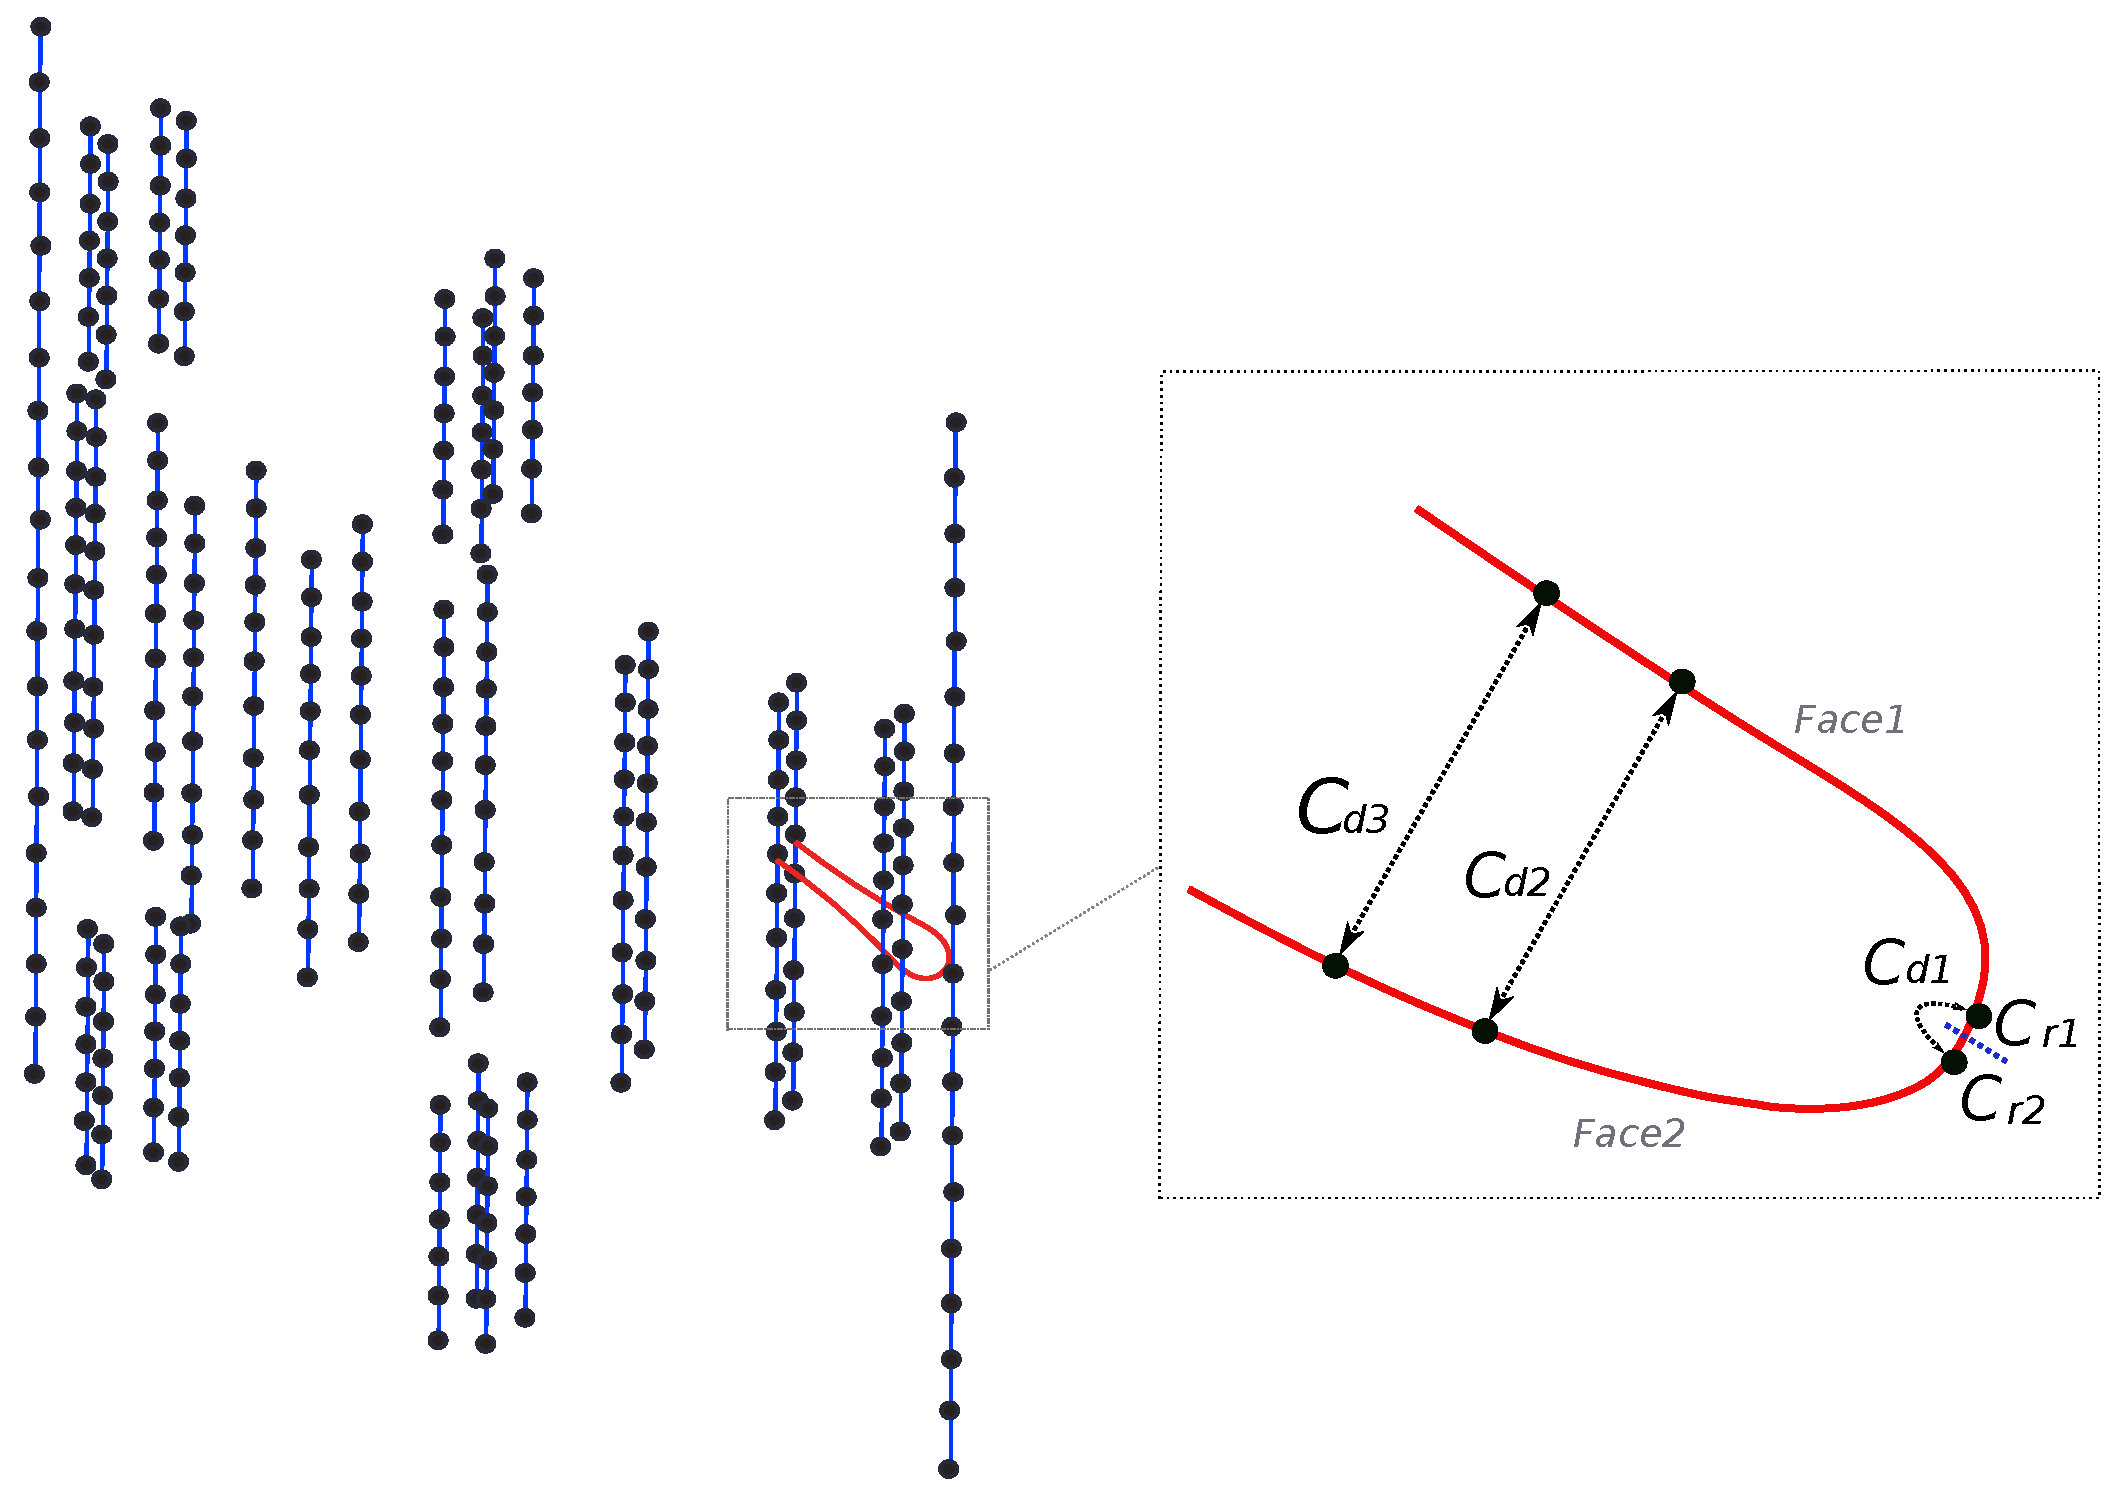
\includegraphics[width = 0.6\textwidth]{images/const3.pdf}
\caption{Left: Constraint visualisation from the STEP file; Right: Constraints computation on the testpoints}
\end{center}
\end{figure}

CAD models are usually constructed from multiple adjacent patches. Therefore, modifications of control points individually on patches can violate (i) patch-continuity (holes between the CAD faces, non-smooth shapes) or (ii) other geometrical constraints. We alleviate this problem by filtering out the shape modes with undesired constraints violations using discrete spaces constructed using test-points (NSPCC approach) \cite{xu13:cad-based},\cite{xu15cad-based}. Conceptually, the approach requires that the constraints are satisfied on the particular set of points defined on the surface (test-points). 

In this work, we propose further development of NSPCC for user-friendly constraints definition. Several methods were devised to accelerate and automate the process of test-point distribution and visualise them.  In Fig. 1. the constraints are deployed in pairs and stored in a coloured STEP format. On each coloured pair, a number of test-points are distributed by means of OCCT, and then composed in the constraint matrix as in \cite{xu15cad-based}. Making use of the OCCT functionality and its differentiated version, the following types of constraints are implemented and also presented in Fig.1.:
\begin{itemize}
\item Cross-patch continuity ($C_{d1}$)
\item Distance $(C_{d2}, C_{d3})$
\item Distance in X, Y, or Z direction
\item Radius of curvature in some point ($C_{r1}, C_{r2}$)
\end{itemize}
In the next section, the results of NURBS-based optimisation with above-mentioned constraints are shown.


\vspace{10pt}
\noindent\underline{Results for the TU Berlin Stator Testcase:}\vspace{0.2em}\newline
The complete description of TU Berlin Stator testcase could be found via \url{http://aboutflow.sems.qmul.ac.uk/events/munich2016/benchmark/testcase3/}. This case represents a typical turbomachinery optimisation problem, subject to a number of geometrical constraints. The corresponding constraint file is shown in Fig. 1. and includes minimal thickness constraint in the middle of the blade, spaces for four bolts (two at the hub and two at the shroud sides), axial chord constraint (Distance in X) and minimal radius for the trailing and the leading edge (Radius of curvature constraint).

\begin{figure}[t!]
  \centering
    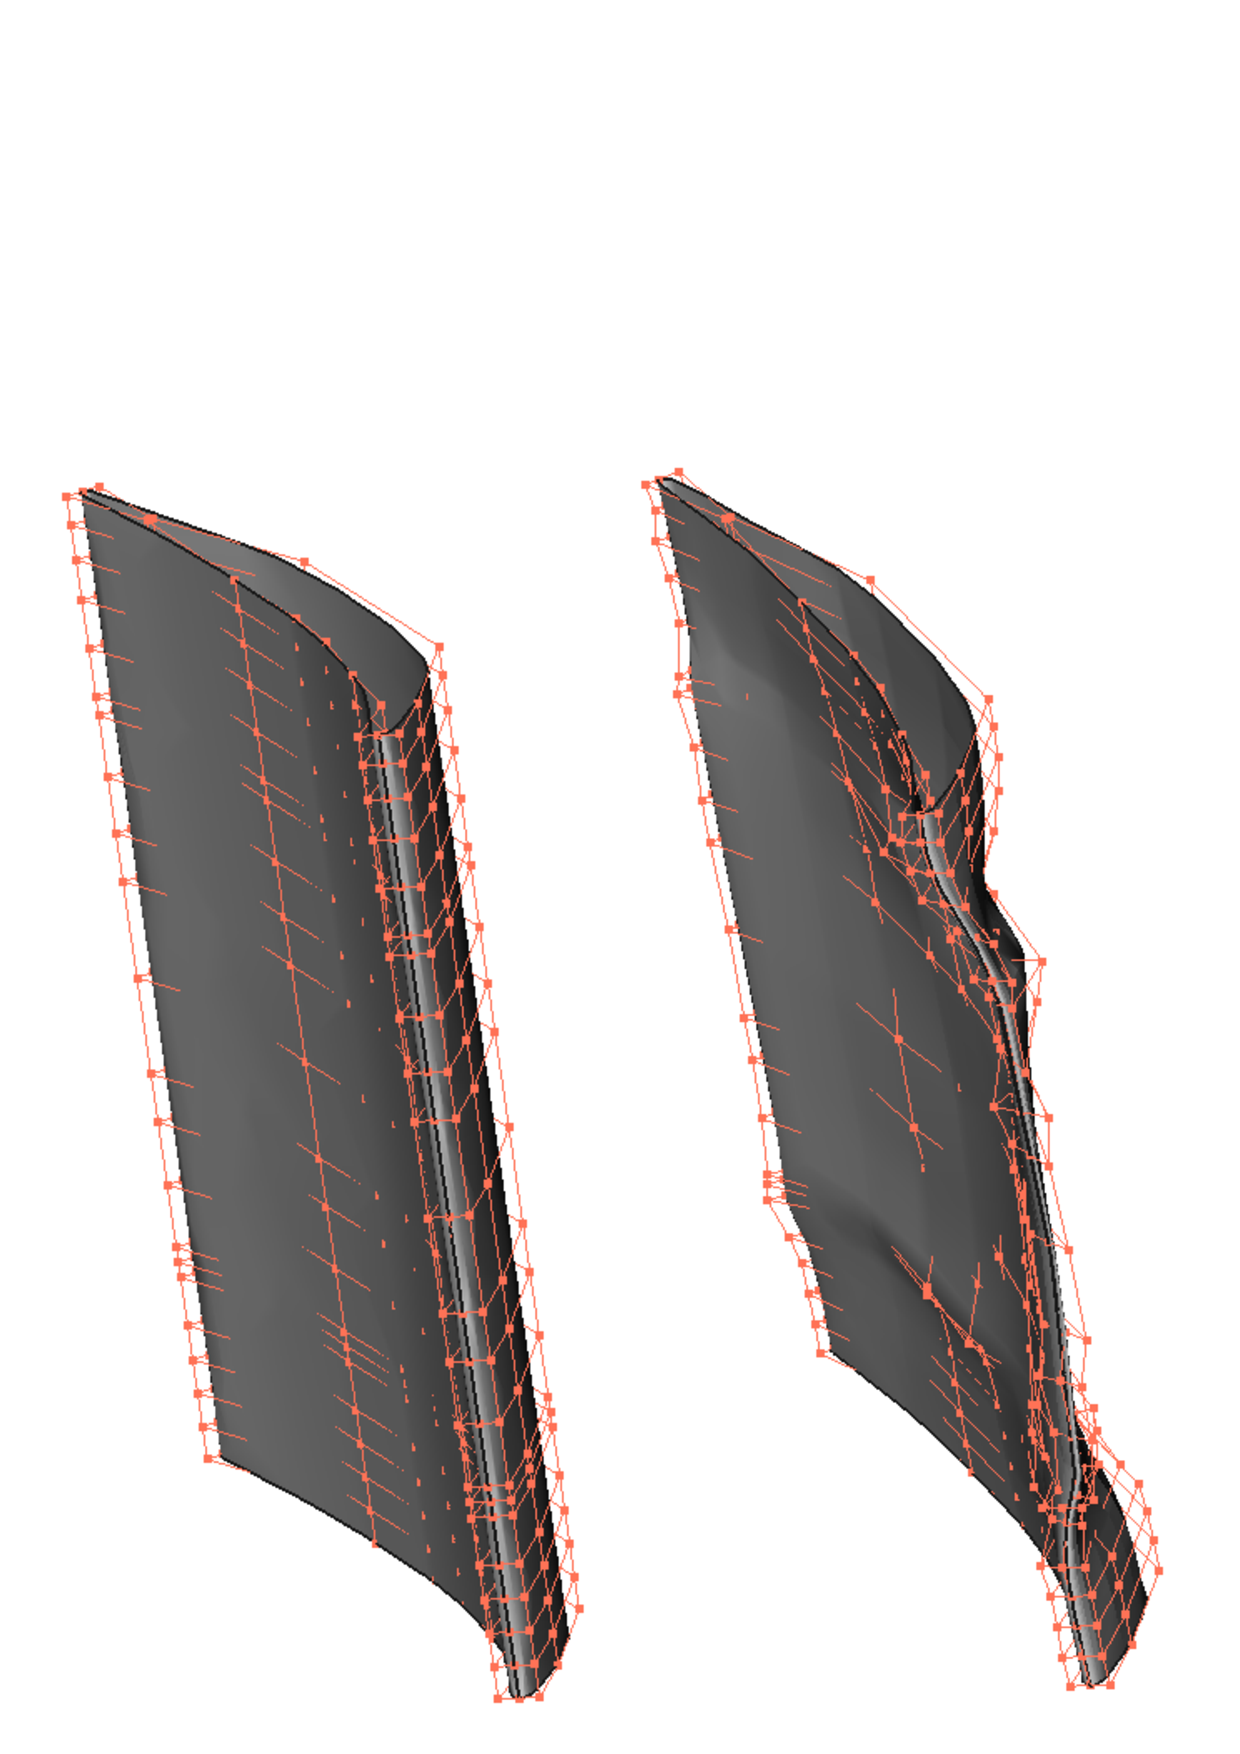
\includegraphics[width=0.5\textwidth, height=200px]{images/blades}
    ~~~
    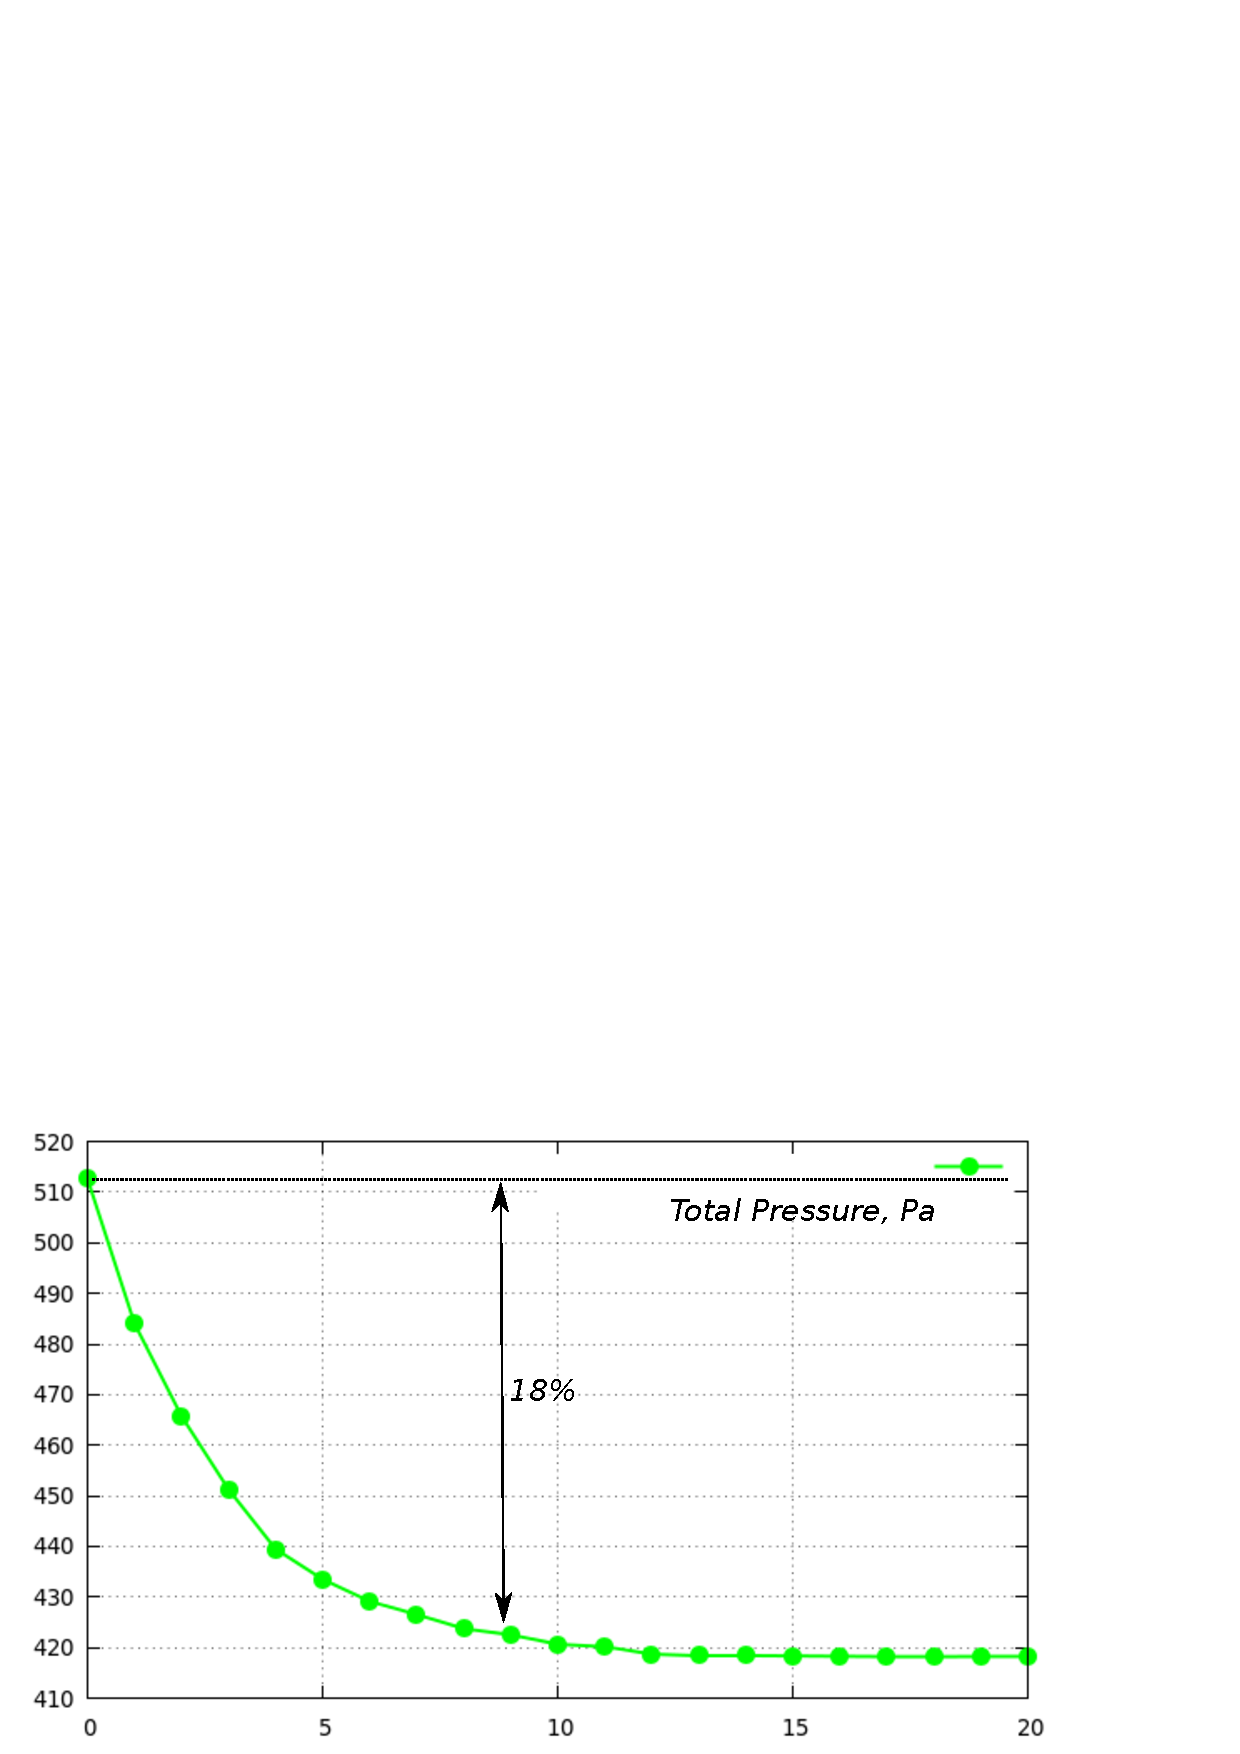
\includegraphics[width=0.45\textwidth, height = 180px]{images/costFunction}
	\caption{Left: Original and Optimised TUB stator blade with NURBS Control Point Net; Right: 20 iterations of Optimisation loop}
    \label{fullmodel}
\end{figure}



With all constraints set, the optimisation is conducted with NSPCC approach to minimise the total pressure loss in the stator at the operating point with 42 degrees of swirl. The results are provided in Fig. 2. and were obtained on the coarse mesh with the STAMPS solver and differentiated OCCT. The changes of NURBS control point net resulted in partial shrinking of the blade, while NSPCC methodology prevented an infraction of the constraints, in general providing 18\% improvement to the cost function.   


\vspace{1em}
\noindent\underline{Conclusions:}\vspace{0.2em}\newline
The use of differentiated CAD-kernel OCCT in combination with adjoint CFD method is showcased for the aerodynamic shape optimisation. The developed CAD tool allows to find optimised designs  and impose geometrical constraints for both parametric models and generally richer NURBS parametrisation spaces with result directly in the CAD format. In the final paper NURBS-based optimisation will be enhanced by automatic design space refinement and it will be compared to a parametric optimisation where the design space consists of conventional turbomachinery parameters.

\vspace{1em}
\noindent\underline{Acknowledgement:}\vspace{0.2em}\newline
This research is a part of the IODA project - Industrial Optimal Design using Adjoint CFD. IODA is \textit{Marie Sklodowska-Curie Innovative Training Network} funded by European Commission under Grant Agreement No.~642959.

\vspace{1em}
\noindent\underline{IMPORTANT NOTES:}\vspace{0.2em}\newline
WE ARE REQUIRED BY CROSSREF TO INCLUDE HYPERLINK INTO EVERY REFERENCE THAT HAS DOI LINKING. PLEASE GO TO: \ULurl{http://www.crossref.org/SimpleTextQuery/}, REGISTER YOUR E-MAIL, CUT AND PASTE THE LIST OF REFERENCES INTO THE BOX, GET THE DOI LINKS AND PASTE THEM INTO YOUR PAPER! THE LINKS SHOULD LOOK LIKE THIS, I.E. USE HTTPS AND DROP THE DX: \ULurl{https://doi.org/10.1080/16864360.2014.881190}


\vspace{1em}
\noindent\underline{References:}\vspace{-1.9em}\newline
\renewcommand{\section}[2]{}
\begin{thebibliography}{9}
\bibitem{auriemma2016optimisation}Auriemma, S.; Banovic, M.; Mykhaskiv, O.; Legrand, H.; M\"uller, J.-D.; Walther, A.: Optimisation of a U-bend using CAD-based adjoint method with differentiated CAD kernel, ECCOMAS Congress, 2016.

\bibitem{jameson88aerodynamic} Jameson, A.: Aerodynamic Design via Control Theory, Journal of Scientific Computing, 3, 1988,  233--260. \ULurl{https://doi.org/10.1007/BF01061285}

\bibitem{xu2015thesis} Xu, S.: CAD-based CFD shape optimisation using discrete adjoint solvers, Ph.D. Thesis, Queen Mary University of London, 2015.

\bibitem{xu15cad-based} Xu, S.; Radford, D.; M\"uller, J.-D.: CAD-based adjoint shape optimisation of a one-stage turbine with geometric constraints, ASME Turbo Expo, 2015.

\bibitem{xu13:cad-based} Xu, S.; Wolfram, J.; M\"uller J.-D.: CAD-based shape optimisation with CFD using a discrete adjoint, International Journal for Numerical Methods in Fluids, 74(3), 2013, 153-168. \ULurl{https://doi.org/10.1002/fld.3844}
\end{thebibliography}



\end{document}
